\g
\chapter{Θεωρητική ανάλυση τεχνητού νευρωνικού δικτύου}
\label{Chapter3}

\section{Χρήση νευρωνικών δικτύων στη στερεοσκοπική όραση}

Η αρχικοποίηση του πίνακα κόστους με διαφορετικές τεχνικές μας βοηθάει να εξάγουμε ένα χρήσιμο συμπέρασμα: η απόδοση της μετρικής ομοιότητας μπορεί να βελτιωθεί αν η σύγκριση δεν βασιστεί στις αρχικές τιμές της φωτεινότητας των υπό σύγκριση χωρίων, αλλά σε ένα πιο αξιόπιστο περιγραφέα της γειτονιάς. Ως αξιόπιστο περιγράφουμε έναν περιγραφέα που είναι όσο το δυνατόν λιγότερο ευάλωτος στα φαινόμενα που προκαλούν αλλοίωση της "ομοιότητας γειτονιάς", όπως αυτά αναλύθηκαν στο προηγούμενο κεφάλαιο \ref{sec:stereo_constraints_violation}. Για παράδειγμα, ο μετασχηματισμός \e census \citep{zabih1994non} \g δημιουργεί τοπικό περιγραφέα που είναι ανεπηρέαστος από τις φωτομετρικές αποκλίσεις. Ταυτόχρονα όμως έχει το μειονέκτημα να δημιουργεί παρόμοιο περιγραφέα από τελείως διαφορετικά είδωλα που τυχαίνει να δημιουργούν γειτονιές με παρόμοια σχέση φωτεινότητας περιφέρειας και κεντρικού \e pixel. \g Η παρατήρηση ότι κάθε μέθοδος έχει διαφορετικά πλεονεκτήματα και αδυναμίες προτρέπει τον συνδυασμό μεθόδων στον υπολογισμό του τελικού κόστους για πιο αξιόπιστα αποτελέσματα, όπως επιτυχημένα υλοποιεί η μέθοδος \e AD-census \g \citep{mei2011building}.

Το πρόβλημα της εξαγωγής του πιο αξιόπιστου τοπικού περιγραφέα είναι ιδιαίτερα σύνθετο. Το εύρος των πιθανών επιλογών είναι χαοτικά μεγάλο και η βέλτιστη λύση είναι αδύνατο να προβλεφθεί από έναν προγραμματιστή. Αυτή η παρατήρηση μας οδηγεί στην αντιμετώπιση του προβλήματος με μεθόδους μηχανικής μάθησης \e (machine learning) \g και πιο συγκεκριμένα με τη χρήση συνελικτικών νευρωνικών δικτύων \e (convolutional neural networks). \g Έτσι δίνεται η δυνατότητα δόμησης ενός αλγορίθμου που θα δημιουργήσει μόνος του τον βέλτιστο περιγραφέα, μαθαίνοντάς τον από τα δεδομένα. Προϋπόθεση για να συμβεί αυτό είναι η ύπαρξη ικανοποιητικά μεγάλων συλλογών δεδομένων με στερεοσκοπικά ζεύγη που θα περιέχουν την πραγματική πληροφορία παράλλαξης. Τέτοιες συλλογές έχουν δημιουργηθεί και είναι διαθέσιμες τα τελευταία χρόνια.

Η αρχικοποίηση του κόστους αντιστοίχησης με χρήση συνελικτικών νευρωνικών δικτύων έχει δοκιμαστεί κυρίως τα τελευταία τρία χρόνια, έχοντας αποδώσει εξαιρετικά αποτελέσματα. Οι \e Zagoruyko, Komodakis \g \cite{zagoruyko2015learning} πρότειναν τρεις διαφορετικές αρχιτεκτονικές νευρωνικών δικτύων για την σύγκριση τετράγωνων περιοχών εικόνας. \ref{fig:zagoruyko} Οι αρχιτεκτονικές τους εφαρμόστηκαν για την επίλυση προβλημάτων στερεοσκοπικής όρασης μεγάλης απόστασης βάσης \e(wide baseline).\g Οι \e Zbontar, Lecun \g \citep{zbontar2016stereo} \ref{fig:jzbontar} πρότειναν επίσης δύο αρχιτεκτονικές για την αρχικοποίηση του κόστους σε πρόβλημα μικρής απόστασης βάσης \e(small baseline).\g Οι \e Luo et. al \g \citep{Luo} \ref{fig:luo}, από την αρχιτεκτονική των οποίων έχει εμπνευστεί κι η παρούσα εργασία, αντιμετώπισαν το πρόβλημα της αρχικοποίησης του κόστους ως πρόβλημα ταξινόμησης πολλαπλών κατηγοριών. Τέλος, οι \e Alex Kendall et al \g \citep{kendall2017end} \ref{fig:kendall} και οι \e Gydaris, Komodakis \g \citep{gidaris2016detect} \ref{fig:gydaris} αντιμετώπισαν το πρόβλημα του υπολογισμού του χάρτη παράλλαξης με χρήση συνελικτικών νευρωνικών δικτύων από την αρχή ως το τέλος. Οπτική αναπαράσταση των γνωστότερων αρχιτεκτονικών που χρησιμοποίηθηκαν για την αρχικοποίηση του πίνακα κόστους παρατίθεται στο παράρτημα \ref{appendix:common_techniques}.

\section{Αρχιτεκτονική νευρωνικού δικτύου}

Προσεγγίζουμε το πρόβλημα της αρχικοποίησης του πίνακα κόστους, ως πρόβλημα ταξινόμησης πολλαπλών κατηγοριών. Κάθε \e pixel \g $\mathbf{p}$ της λήψης αναφοράς αντιστοιχίζεται (ταξινομείται) σε μία τιμή (κατηγορία) του συνόλου $\{0,1,2,\ldots,\mathtt{max\_disparity}\}$. Το νευρωνικό δίκτυο χωρίζεται σε δύο μέρη, το συνελικτικό δίκτυο το οποίο αναλαμβάνει την εξαγωγή του τοπικού περιγραφέα και το δίκτυο απόφασης στο οποίο υπολογίζεται η τιμή του κόστους ομοιότητας σε κάθε θέση, όπως φαίνεται στο σχήμα \ref{fig:neural_net_arch}.

\begin{figure}
	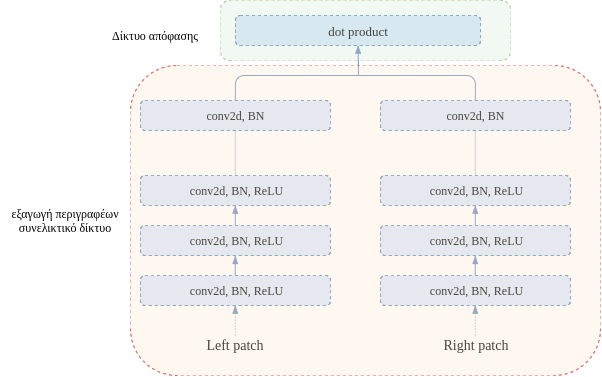
\includegraphics[width=0.9\textwidth]{neural_net_arch.png}
	\caption{Αρχιτεκτονική νευρωνικού δικτύου.}
	\label{fig:neural_net_arch}
\end{figure}

\subsection{Εξαγωγή τοπικών περιγραφέων - Συνελικτικό νευρωνικό δίκτυο}

Στόχος της εξαγωγής τοπικού περιγραφέα είναι η αντιστοίχηση του τετράγωνου χωρίου πέριξ του σημείου ενδιαφέροντος $\mathbf{p}$, δηλαδή της γειτονιάς $N_p$, σε ένα διάνυσμα το οποίο συμβολίζουμε $\mathbf{Ι_{descriptor}}(\mathbf{p})$. Το μέγεθος της πλευράς της τετράγωνης γειτονιάς $\mathtt{patch\_size}$ και το μέγεθος του τελικού διανύσματος $\mathtt{f\_maps}$ είναι ελεύθερες παράμετροι προς επιλογή. Επομένως:

$$\mathbf{Ι_{descriptor}}(\mathbf{p}) = f_{desc}(N_p)$$
$$N_p \in \mathbb{R}^{\mathtt{patch\_size}^2}, \mathbf{Ι_{descriptor}}(\mathbf{p}) \in \mathbb{R}^{\mathtt{f\_maps}}$$

Κάθε μπλοκ του συνελικτικού νευρωνικού δικτύου απαρτίζεται από τα εξής επίπεδα:
\begin{itemize}
	\item \textbf{Δισδιάστατη συνέλιξη}: Συνέλιξη με $\mathtt{f\_maps}$ φίλτρα διαστάσεων $[\mathtt{kernel\_size} \times \mathtt{kernel\_size} \times \mathtt{f\_maps}]$\footnote{Εκτός από το πρώτο μπλοκ, στο οποίο το φίλτρο συνέλιξης έχει διάσταση $\mathtt{kernel\_size} \times \mathtt{kernel\_size} \times 1$, καθώς δέχεται ως είσοδο \e grayscale \g τετράγωνο χωρίο διάστασης $\mathtt{patch\_size} \times \mathtt{patch\_size} \times 1$}. Η συνέλιξη εφαρμόζεται χωρίς \e zero padding \g στον πίνακα εισόδου. Συμβολίζουμε την πράξη ως:
	\e $$y_{conv2d} = \mathbf{conv2d}(x,h)$$ \g
	
	\item \textbf{Πόλωση:} Στο αποτέλεσμα της συνέλιξης του σήματος εισόδου με το κάθε φίλτρο προστίθεται ένας όρος (πόλωση), μετατρέποντας την συνολική πράξη σε μετασχηματισμό \e affine. \g
	
	$$y_{b} = y_{conv2d} + b$$

	\item \textbf{Κανονικοποίηση δέσμης \e (batch normalization):} \citep{ioffe2015batch} \g Η κανονικοποίηση δέσμης αφήνει αμετάβλητες τις διαστάσεις του εισερχόμενου πίνακα, επηρεάζοντας μόνο την εσωτερική του στατιστική. Αναλυτική περιγραφή της μεθόδου και των σκοπών που επιτελεί δίνεται στο παράρτημα \ref{appendix:BN}.
	
	$$y_{BN} = BN(y_b)$$
	\item \textbf{Συνάρτηση γραμμικού ανορθωτή \e (Rectified Linear Unit - ReLU):}\g Εισάγει την απαραίτητη μη γραμμικότητα μέσω της πράξης \e $\text{ReLU}(x) = max(0,x)$\g σε κάθε τιμή του πίνακα εισόδου.
\end{itemize}

Η παραπάνω δομή επιπέδων επαναλαμβάνεται διαδοχικά $\mathtt{num\_conv\_layers}$ φορές. Έπειτα από κάθε μπλοκ, οι χωρικές διαστάσεις του χωρίου μειώνονται κατά $\dfrac{\mathtt{kernel\_size - 1}}{2}$. Στο τέλος ολόκληρου του συνελικτικού νευρωνικού δικτύου, ο πίνακας που θα προκύψει θα έχει διαστάσεις $[1 \times 1 \times \mathtt{f\_maps}]$ κι ουσιαστικά θα είναι ο τοπικός περιγραφέας του χωρίου που δόθηκε ως είσοδος στο δίκτυο.

\subsection{Δίκτυο απόφασης}

Στόχος του δικτύου απόφασης είναι η εκτίμηση της ομοιότητας των δύο περιγραφέων, που αναλογούν στα δύο υπό σύγκριση χωρία. Η εκτίμηση αυτή είναι το αποτέλεσμα μια συνάρτησης $f_{comp}$, που θα δέχεται ως είσοδο τους δύο τοπικούς περιγραφείς $\mathbf{Ι}_{descriptor}^L(\mathbf{p})$, $\mathbf{Ι}_{descriptor}^R(\mathbf{q})$ και θα επιστρέφει μια εκτίμηση ομοιότητας:
	
	$$f_{comp}: \mathbb{R}^{2 \times \mathtt{f\_maps}} \rightarrow \mathbb{R}$$
	$$s = f_{comp}(\mathbf{Ι}_{descriptor}^L\mathbf{p}, \mathbf{Ι}_{descriptor}^R\mathbf{q})$$

Η επιλογή της συνάρτησης αυτής μπορεί να γίνει με δύο τρόπους:

\begin{itemize}
	\item Με την εφαρμογή μιας προαποφασισμένης συνάρτησης $f_{comp}$ όπως η μέση απόλυτη διαφορά, η μέση τετραγωνική διαφορά, το εσωτερικό γινόμενο ή η ομοιότητα συνημιτόνου.
	\item Με την χρήση μηχανικής μάθησης για την εκμάθηση της βέλτιστης συνάρτησης $f_{comp}$ από τα δεδομένα. Στην περίπτωση, μια ενδεδειγμένη λύση είναι η εκπαίδευση ενός "πλήρως συνδεδεμένου" \e (fully connected) \g τεχνητού νευρωνικού δικτύου.
\end{itemize}

\subsubsection*{Ανάλυση της χρήσης τεχνητού νευρωνικού δικτύου ως δίκτυο απόφασης} 

\begin{itemize}
	\item Η εκπαίδευση ενός νευρωνικού δικτύου για την εκτίμηση της ομοιότητας αποτελεί την βέλτιστη επιλογή με κριτήριο την ακρίβεια. Η επιλογή αυτή δίνει τη δυνατότητα στο δίκτυο να "μάθει" από τα δεδομένα την βέλτιστη συνάρτηση $f_{comp}$ που θα περατώνει τον σκοπό της εκτίμησης ομοιότητας των δύο διανυσμάτων εισόδου. 
	\item Από πλευράς ταχύτητας, η βέλτιστη επιλογή είναι η χρήση μιας προαποφασισμένης συνάρτησης, όπως για παράδειγμα το εσωτερικό γινόμενο. Η σύγκριση εκτελείται σειριακά $\mathtt{max\_disparity} + 1$ φορές για κάθε σημείο της εικόνας, επομένως αν ο χρόνος περάτωσης της συνάρτησης σύγκρισης είναι $t_f$, ο συνολικός χρόνος θα είναι $(\mathtt{max\_disparity} + 1)\times t_f$. Η χρήση μιας απαιτητικής υπολογιστικά συνάρτησης με πολύ μεγάλο $t_f$, όπως το "απόλυτα συνδεδεμένο" νευρωνικό δίκτυο αυξάνει πολύ έντονα το χρόνο εκτέλεσης. Αντιθέτως, μια συνάρτηση όπως το εσωτερικό γινόμενο, αφενός λόγω πολύ μικρού $t_f$ κρατάει τον συνολικό χρόνο σε χαμηλά επίπεδα ακόμη και για μεγάλο $\mathtt{max\_disparity}$ αφετέρου μπορεί να υλοποιηθεί παράλληλα σε κάρτα γραφικών.
	\item H εκπαίδευση του συνελικτικού δικτύου και του δικτύου απόφασης γίνεται ενιαία. Αυτό προϋποθέτει τη χρήση μιας παραγωγίσιμης συνάρτησης $f_{comp}$, ώστε να μπορεί να εφαρμοστεί πάνω της ο κανόνας της οπισθοδιάδοσης \e(back propagation). \g
\end{itemize}

Παρατηρώντας ότι τα αποτελέσματα είναι ικανοποιητικά με χρήση μιας πράξης εσωτερικού γινομένου στα δύο διανύσματα, με ταυτόχρονη κατακόρυφη μείωση της υπολογιστικής πολυπλοκότητας το προτιμούμε σε σχέση με την εκπαίδευση ενός "απόλυτα συνδεδεμένου" νευρωνικού δικτύου.

\section{Εκπαίδευση νευρωνικού δικτύου}

\subsection{Δημιουργία σετ εκπαίδευσης νευρωνικού δικτύου}

Στο παράρτημα \ref{appendix:stereo_dataset} παραθέτουμε εκτενή ανάλυση των χαρακτηριστικών που διέπουν τις υπάρχουσες στερεοσκοπικές συλλογές.

Η δημιουργία του σετ εκπαίδευσης βασίζεται στις εικόνες της στερεοσκοπικής συλλογής \e KITTI \g με την ακόλουθη προεπεξεργασία σε κάθε εικόνα:\footnote{όλες οι εικόνες στις οποίες αναφερόμαστε είναι \e grayscale \g}

\begin{itemize}
	\item Μετατροπή τους σε εικόνες μηδενικής μέσης τιμής. Στην αρχική τους μορφή όλες οι εικόνες είναι πίνακες ακεραίων αριθμών $I \in \mathbb{Z}: \{ 0 \leqslant I \leqslant 255 \}$. Εφαρμόζουμε την πράξη:
	
	$$\mu = \dfrac{1}{Μ \times N} \cdot \sum_{\mathbf{p}} I(\mathbf{p})$$
	
	$$I^{\mathbf{z\_m}} = I - \mu$$ 
	Ο νέος πίνακας έχει σύνολο τιμών το σύνολο των πραγματικών αριθμών $I^{\mathbf{z\_m}} \in \mathbb{R}$.
	\item Κανονικοποίηση \e (normalization) \g μέσω της μετατροπής τους σε εικόνες μοναδιαίας διακύμανσης. Εφαρμόζουμε την πράξη:
	
	$$\sigma^2 = \dfrac{1}{Μ \times N} \cdot \sum_{\mathbf{p}} I_{\mathbf{z\_m}}(\mathbf{p})$$
	$$I^{\mathbf{unit\_var}} = \dfrac{I^{\mathbf{zm}} }{ \sigma }$$
\end{itemize}

\textbf{Επισημάνσεις:}
\begin{itemize}
	\item Η μετατροπή σε εικόνες μηδενικής μέσης τιμής και μοναδιαίας διακύμανσης γίνεται στο σύνολο της εικόνας κι όχι στο κάθε τετράγωνον χωρίο \e (patch) \g που θα εξαχθεί κατά τη δημιουργία του σετ εκπαίδευσης. Αυτό συμβαίνει διότι κατά την εκτέλεση του αλγορίθμου θα προωθούμε ολόκληρη την εικόνα στο δίκτυο (όχι κάθε χωρίο ξεχωριστά) και θέλουμε το δίκτυο να εκπαιδευτεί σε δεδομένα ίδιας στατιστικής με αυτά που θα αντιμετωπίσει κατά τον έλεγχο \e (testing). \g 
	\item Οι υπολογισμοί της μέσης τιμής και της τυπικής απόκλισης γίνεται σε κάθε εικόνα ξεχωριστά. Δεν ακολουθούν τον ορισμό της κανονικοποίησης που ορίζει την κανονικοποίηση της κάθε διάστασης (κάθε ξεχωριστό \e pixel \g στην προκειμένη) κατά μήκος όλου του σετ εκπαίδευσης. Αυτή η εναλλακτική μορφή κανονικοποίησης είναι η πιο διαδεδομένη μέθοδος προεπεξεργασίας όταν η συλλογή περιλαμβάνει εικόνες.
\end{itemize}

Συμβολίζουμε με

\e
$$
<\mathcal{P}_{n \times n}^L(\mathbf{p}), \mathcal{P}_{( \texttt{max\_disparity} + n) \times n}^R(\mathbf{q}), \text{label}>
$$
\g

κάθε εγγραφή του σετ εκπαίδευσης, όπου:

\begin{itemize}
	\item $\mathcal{P}_{n \times n}^L(\mathbf{p})$, είναι το τετράγωνο χωρίο διάστασης $n \times n$ της αριστερής εικόνας με κέντρο το σημείο $\mathbf{p}$
	\item \e $\mathcal{P}_{( \texttt{max\_disparity} + n) \times n}^R(\mathbf{q})$, \g είναι το παραλληλόγραμμο χωρίο διάστασης \e $\texttt{max\_disparity} + n) \times n$ \g της δεξιάς λήψης. Ουσιαστικά περιέχει τα τετράγωνα χωρία που ορίζονται γύρω από όλες τις υποψήφιες θέσεις παράλλαξης $\mathbf{p-d}$.
	\item \e $\text{label}$, \g συμβολίζουμε ένα διάνυσμα \e $\mathtt{max\_disparity+1}$ \g θέσεων το οποίο λαμβάνει τιμές με τον ακόλουθο κανόνα:
	
	\begin{equation*}
	label[i] = \begin{cases}
		0.5 & \text{εάν} \:i = true\_disparity\\
		0.2 & \text{εάν} \: |i - true\_disparity| = 1\\
		0.05 & \text{εάν} \: |i - true\_disparity| = 2\\
		0 & \text{αλλιώς}
	\end{cases}
\end{equation*}
	
\end{itemize}

Ο λόγος που επιλέγουμε αυτήν την κατανομή στο διάνυσμα \e label \g, αντί του συνηθισμένου \e one-hot encoding \g οφείλεται στο ότι επιθυμούμε το δίκτυο να υπολογίζει μικρό κόστος ομοιότητας όχι μόνο στην σωστή παράλλαξη, αλλά και στις γειτονικές περιοχές εντός του ορίου $\pm 2$ θέσεων.

Αναλυτική περιγραφή με αλγοριθμικές λεπτομέρειες της δημιουργίας των παραδειγμάτων εκπαίδευσης δίνεται στο παράρτημα \ref{appendix:dataset_creation}.

Ένα παράδειγμα εγγραφής του σετ εκπαίδευσης φαίνεται στο σχήμα \ref{kitti2012_multi_class_dataset}. Δημιουργούνται περίπου $8\cdot10^4\times\dfrac{\text{εγγραφές}}{\text{εικόνα}}$ οπότε το συνολικό σετ εκπαίδευσης περιέχει περίπου $32\times10^6$ εγγραφές.
\begin{figure}
	\centering
	\begin{subfigure}{\textwidth}
	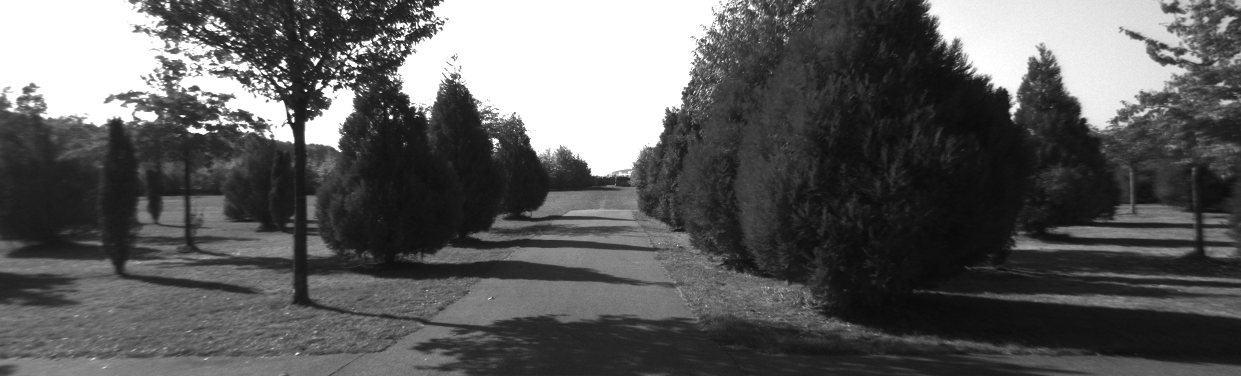
\includegraphics[width=\textwidth]{kitti2012_im9.png}
	\end{subfigure}
	\label{fig:kitti2012_imL_9}
	\caption{Αριστερή εικόνα $I^L$ στερεοσκοπικού ζεύγους της συλλογής \e KITTI (2012) \g}	
	\begin{subfigure}{.3\textwidth}
		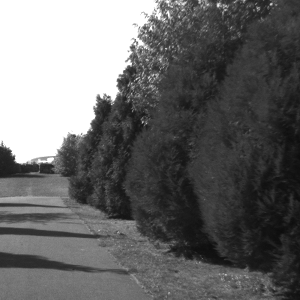
\includegraphics[width=\textwidth, height=4cm]{kitti2012_im9_lcrop.png}
		\caption{\e $\mathcal{P}_{150 \times 150}^L(163,731)$ \g}
	\end{subfigure}
		\begin{subfigure}{.69\textwidth}
		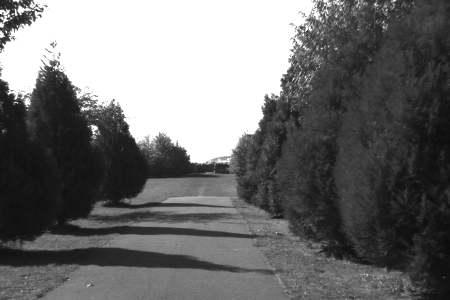
\includegraphics[width=\textwidth, height=4cm]{kitti2012_im9_rcrop.png}
		\caption{\e $\mathcal{P}_{( 150 + 150) \times 150}^R(163,701)$ \g}
	\end{subfigure}
	\label{kitti2012_multi_class_dataset}
	\caption[αεκ]{παράδειγμα δημιουργίας εγγραφής στο σετ εκπαίδευσης ταξινόμησης πολλαπλών κατηγοριών. H επιλογή μεγέθους ορθογώνιου χωρίου $150\times150$ δεν είναι ρεαλιστική, αλλά έγινε για να είναι εύληπτη η εικόνα. Στην πραγματικότητα το μέγεθος του χωρίου δεν υπερέβη ποτέ τα \e $n=40 \text{pixels}$ \g στους πειραματισμούς μας.}
\end{figure}

\subsection{Υπολογισμός συνάρτησης κόστους προς ελαχιστοποίηση}

Συμβολίζουμε ως $\Theta$ το σύνολο των εκπαιδεύσιμων παραμέτρων του νευρωνικού δικτύου. Παρακάτω αναλύουμε πως δομείται η συνάρτηση κόστους $J_X(\theta)$ την οποία θα ελαχιστοποιήσουμε.

Κάθε εγγραφή του σετ εκπαίδευσης συμβολίζεται ως

\e
$$
<\mathcal{P}_{n \times n}^L(\mathbf{p}), \mathcal{P}_{( \texttt{max\_disparity} + n) \times n}^R(\mathbf{q}), \text{label}>
$$
\g

Το συνελικτικό νευρωνικό δίκτυο αποτελείται από δύο όμοιους κλάδους (αρχιτεκτονική σιαμαίων δικτύων). Ο ένας κλάδος δέχεται ως είσοδο το τετράγωνο χωρίο διάστασης $[\mathtt{patch\_size} \times \mathtt{patch\_size} \times 1]$ που αναλογεί στο $\mathcal{P}_{n \times n}^L(\mathbf{p})$ και ο άλλος κλάδος το παραλληλόγραμμο διάστασης $[(\mathtt{patch\_size} + \mathtt{max\_disparity}) \times \mathtt{patch\_size} \times 1]$ που αναλογεί στο $\mathcal{P}_{( \mathtt{max\_disparity} + n) \times n}^R(\mathbf{q})$. Στην έξοδο του συνελικτικού δικτύου λαμβάνουμε:

\begin{itemize}
	\item τον περιγραφέα $\mathbf{Ι}_{descriptor}^L(\mathbf{p})$ του σημείου $\mathbf{p}$ της αριστερής λήψης. Το διάνυσμα αυτό αναπαρίσταται από έναν πίνακα διάστασης $\mathtt{f\_maps}$.
	\item τους περιγραφείς $\mathbf{Ι}_{descriptor}^R(\mathbf{p-d})$ όλων των υποψήφιων "αντίστοιχων σημείων" της δεξιάς λήψης. Το διάνυσμα αυτό αναπαρίσταται από έναν πίνακα διάστασης $(\mathtt{max\_disparity} + 1)\times \mathtt{f\_maps}$.
\end{itemize}

Η διαδοχή των βημάτων και των διαστάσεων των πινάκων φαίνεται συμπυκνωμένα στον πίνακα \ref{tbl:train_model}.

Εφαρμόζουμε την πράξη του εσωτερικού γινομένου $(\mathtt{max\_disparity} + 1)$ φορές, υπολογίζοντας έτσι το διάνυσμα $\mathbf{score} \in \mathbb{R}^\mathtt{max\_disparity+1}$. Το διάνυσμα $\mathbf{score}$ περιέχει το σκορ ομοιότητας του χωρίου αναφοράς με το αντίστοιχο χωρίο της έτερης λήψης, σε κάθε πιθανή θέση παράλλαξης.

\begin{table}[t]
\e
\centering
\resizebox{\linewidth}{!}{
\begin{tabular}{l|l|c|c}
\e Block \g & \g Περιγραφή Επιπέδων & \g $\mathcal{P}_{n \times n}^L(\mathbf{p})$ & \g $\mathcal{P}_{( \mathtt{max\_disparity} + n) \times n}^R(\mathbf{q})$ \e \\ \hline \hline
%
\multicolumn{3}{c}{\textbf{Local descriptors extraction \g(Εξαγωγή περιγραφέων)\e}} \\ \hline
\multicolumn{3}{c}{\textbf{Siamese network \g(Σιαμαίο δίκτυο)\e}} \\ \hline
\g Eίσοδος \e &  &  $n \times n \times 1$ & $(d+n) \times n \times 1$\\ \hline
1 & conv2d, F=64 & $(n-x) \times (n-x) \times F$ & $(d+n-x) \times (n-x) \times F$\\
2 & conv2d, F=64 & $(n-2x) \times (n-2x) \times F$ & $(d+n-2x) \times (n-2x) \times F$\\
$i$ & conv2d, F=64 & $(n-ix) \times (n-ix) \times F$ & $(d+n-ix) \times (n-ix) \times F$\\
\vdots &  \qquad \qquad  \vdots  & \vdots & \vdots		         \\
$\sfrac{n-1}{x}$ & conv2d, F=64 & $1 \times 1 \times F$ & $(d+1) \times 1 \times F$\\ \hline
\g Έξοδος & & $F$ & $(d+1) \times F$\\ \hline \hline
%
\end{tabular}}
	\caption{\g Περίληψη επιπέδων δικτύου κι αντίστοιχων διαστάσεων πινάκων κατά την εκπαίδευση. Ως $d$ συμβολίζεται η μέγιστη παράλλαξη $\mathtt{max\_disparity}$, ως $x$ την μείωση των διαστάσεων του πίνακα εισόδου κατά τη συνέλιξη $\dfrac{\mathtt{kernel\_size}-1}{2}$, ως $n$ τη διάσταση του χωρίου εισόδου $\mathtt{patch\_size}$.}
	\label{tbl:train_model}
\g
\end{table}

Η μετατροπή των τιμών του διανύσματος $\mathbf{score} \in \mathbb{R}^\mathtt{max\_disparity+1}$ σε πιθανότητες γίνεται μέσω της συνάρτησης \e softmax: \g

$$p_d = \dfrac{e^{\mathbf{score}_d}}{\sum_{d = 0}^{\mathtt{max\_disparity}} e^{\mathbf{score}_d} }, \quad \forall d \in [0, \mathtt{max\_disparity+1}] $$

Μέσω αυτής της πράξης δημιουργείται ένα διάνυσμα πιθανοτήτων $\mathbf{poss} \in \mathbb{R}^\mathtt{max\_disparity+1}$, με τιμές εντός του διανύσματος $[0,1]$ το άθροισμα των οποίων ισούται με την μονάδα $\sum_{d=0}^\mathtt{max\_disparity} p_d = 1$.

Ορίζουμε συνάρτηση εντροπίας ως:
\e
$$H = \sum_{d = 0}^{\mathtt{max\_disparity}} \text{label(d)} log (\mathbf{poss}(d))$$
\g

Αναπαρίστουμε την συνάρτηση κόστους του κάθε παραδείγματος εκπαίδευσης ως $H_j$. Σε κάθε βήμα εκπαίδευσης το συνολικό κόστος υπολογίζεται στο σύνολο της δέσμης εκπαίδευσης:

$$L = \sum_{j = 0}^{\mathtt{batch\_size}} H_j$$

κι είναι μια τιμή που εξαρτάται από:
\begin{itemize}
	\item τις εκπαιδεύσιμες παραμέτρους του δικτύου, έστω ότι τις συμβολίζουμε με $\Theta$
	\item τα παραδείγματα της δέσμης εκπαίδευσης με τις αντίστοιχες ετικέτες τους \e(labels)\g, έστω ότι τα συμβολίζουμε ως $X$
\end{itemize}

Υπολογίζουμε σφάλμα γενίκευσης:

$$R = \lambda \sum_i \Theta_i^2$$

Η ολική συνάρτηση κόστους είναι το άθροισμα της εντροπίας υπολογισμένη στην δέσμη παραδειγμάτων $X$ και του σφάλματος γενίκευσης:

$$J_X(\Theta) = L + R$$

Θεωρούμε δεδομένα τα παραδείγματα της δέσμης εκπαίδευσης κι αντιμετωπίζουμε ως μεταβαλλόμενο μέγεθος μόνο τις παραμέτρους του δικτύου(βάρη των φίλτρων, πολώσεις, συντελεστές $\gamma, \beta$ της κανονικοποίησης δέσμης). Η συνάρτηση κόστους επομένως είναι μια συνάρτηση:

$$J_X(\Theta) \: : \mathbb{R}^n \rightarrow \mathbb{R}$$

Στόχος μας είναι να βρούμε τις τιμές εκείνες των παραμέτρων $\Theta$ που φτάνουν "κοντά" στην ελάχιστη τιμή της $J$:

\begin{equation}
	|J_X^{optimal}(\Theta)-J_X^{min}(\Theta)|< \varepsilon
	\label{eq:total_minima}
\end{equation}

Στο παράρτημα \ref{appendix:minimum_explanation} αναλύεται γιατί στοχεύουμε στον υπολογισμό ενός διανύσματος $\Theta$ στην γειτονιά του $\Theta_{min}$.

\subsection{Αρχικοποίηση των εκπαιδεύσιμων παραμέτρων του δικτύου}

Η συνάρτηση $J_X(\Theta)$ είναι:
\begin{itemize}
	\item συνεχής
	\item μη-κυρτή \e(non-convex)\g \ref{fig:convex}
	\item μη κοίλη \e(non-concave)\g 
\end{itemize} 

Η δεύτερη και τρίτη ιδιότητα δυσκολεύουν την προσπάθεια εύρεσης του ολικού ελάχιστου. Δεν υπάρχει κανένα εχέγγυο ότι ακολουθώντας την διεύθυνση της κλίσης της συνάρτησης κόστους θα οδηγηθούμε στο ολικό ελάχιστο. Αντίθετα είναι σχεδόν βέβαιο ότι η μέθοδός μας θα "παγιδευτεί" σε κάποιο από τα τοπικά ελάχιστα. Αυτό ταυτόχρονα σημαίνει ότι για διαφορετικές αρχικές τιμές παραμέτρων το τελικό αποτέλεσμα θα είναι πιθανότατα διαφορετικό, όπως φαίνεται στην εικόνα \ref{fig:non_convex_random}.

H πειραματικά επιβεβαιωμένη παρατήρηση που διευκολύνει την επίλυση του προβλήματος εντοπίζει ότι η συνάρτηση $J_X(\Theta)$ εμφανίζει σχετικά μικρή απόκλιση ανάμεσα στα τοπικά και στο ολικό της ελάχιστο. Η προσέγγιση ενός τοπικού ελάχιστου δεν θα δώσει ιδιαίτερα χειρότερο αποτέλεσμα από την προσέγγιση του ολικού ελαχίστου. Η παρατήρηση αυτή (μη αποδεδειγμένη μαθηματικά) δίνει αρκετές πιθανότητες η εκπαίδευση του δικτύου να σημειώσει πρόοδο και να καταλήξει σε ένα ικανοποιητικό αποτέλεσμα, εκκινώντας από αρκετά διαφορετικά σημεία. Παρ' όλα αυτά, η αρχικοποίηση των παραμέτρων κατέχει σημαντικό ρόλο στην εξέλιξη της εκπαίδευσης του δικτύου.

Αρχικοποιούμε το δίκτυο με τις ακόλουθες κατανομές:
\begin{itemize}
	\item οι τιμές των φίλτρων του νευρωνικού δικτύου (βάρη) αρχικοποιούνται με την κατανομή που πρότειναν οι \e He et. al \g \citep{He_2015_ICCV}. Η κατανομή αυτή είναι μια κανονική γκαουσιανή την οποία κλιμακώνουμε με την τιμή $\sfrac{2}{n}$, όπου $n$ ο αριθμός των νευρώνων του προηγούμενου επιπέδου. Έτσι εξασφαλίζουμε ότι η κατανομή έχει διακύμανση $\sfrac{2}{n}$ κι η διακύμανση της κατανομής στην έξοδο του συγκεκριμένου επιπέδου θα είναι μοναδιαία.
	\item οι πολώσεις αρχικοποιούνται με μηδενικές τιμές
	\item οι κλιμακώσεις $\gamma$ των επιπέδων κανονικοποίησης δέσμης με μονάδα
	\item οι μετατοπίσεις $\beta$ των επιπέδων κανονικοποίησης δέσμης με μηδενικές τιμές
\end{itemize}

Οι εκπαιδεύσιμες(μεταβλητές) παράμετροι του δικτύου φαίνονται αναλυτικά στον πίνακα \ref{tbl:trainable_parameters}.


\begin{figure}
	\centering
	\begin{subfigure}{0.49\textwidth}
		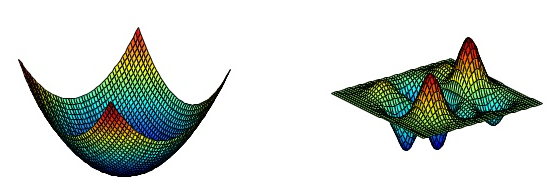
\includegraphics[width=\textwidth]{convex_vs_non_convex.png}
		\caption{Παράδειγμα κυρτής (αριστερά) και μη-κυρτής (δεξιά) συνάρτησης.}
		\label{fig:convex}
	\end{subfigure}
	\begin{subfigure}{0.49\textwidth}
		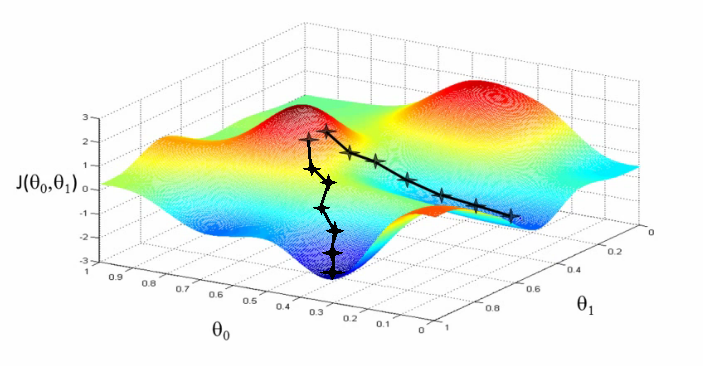
\includegraphics[width=\textwidth]{non_convex_random.png}
		\caption{Διαφορετική αρχικοποίηση οδηγεί τον αλγόριθμο "απότομης καθόδου" σε διαφορετικό τελικό αποτέλεσμα.}
		\label{fig:non_convex_random}
	\end{subfigure}	
\end{figure}

\begin{table}[t]
\e
\begin{tabular}{l|l|l}
\hline \hline
\multicolumn{3}{c}{\textbf{\g Συνελικτικό νευρωνικό δίκτυο - Εξαγωγή τοπικού περιγραφέα\e}} \\ \hline
& \g Επίπεδο & \g Εκπαιδεύσιμες παράμετροι \\ \hline \hline
%
\multicolumn{3}{c}{\textbf{block 1}} \\ \hline
1 & \textbf{conv2d} & $\mathtt{patch\_size}^2 \times 1 \times \mathtt{f\_maps}$ \\
2 & \textbf{biases} & $\mathtt{f\_maps}$ \\
3 & \textbf{BN} & $2 \times \mathtt{f\_maps}$ \\
4 & \textbf{ReLU} & $0$ \\ \hline \hline
%
\multicolumn{3}{c}{\textbf{block 2}} \\ \hline
1 & \textbf{conv2d} & $\mathtt{patch\_size}^2 \times \mathtt{f\_maps}^2$\\
2 & \textbf{biases} & $\mathtt{f\_maps}$ \\
3 & \textbf{BN} & $2 \times \mathtt{f\_maps}$ \\
4 & \textbf{ReLU} & $0$ \\ \hline \hline
%
\vdots & \vdots & \vdots \\ \hline 
%
\multicolumn{3}{c}{\textbf{block $\mathtt{n\_blocks}$}} \\ \hline
1 & \textbf{conv2d} & $\mathtt{patch\_size}^2 \times \mathtt{f\_maps}^2$\\
2 & \textbf{biases} & $\mathtt{f\_maps}$ \\
3 & \textbf{BN} & $2 \times \mathtt{f\_maps}$ \\ \hline\hline
%
\multicolumn{3}{c}{\textbf{\g Δίκτυο απόφασης}} \\ \hline
1 & \textbf{dot product} & $0$\\ \hline \hline
%
\multicolumn{3}{c}{\textbf{\g Σύνολο}} \\ \hline
\multicolumn{3}{c}{$(\mathtt{patch\_size}^2 \times \mathtt{f\_maps}^2 + 3\mathtt{f\_maps})\mathtt{n\_blocks}$}
\end{tabular}
	\caption{\g Περίληψη εκπαιδεύσιμων παραμέτρων του νευρωνικού δικτύου.}
	\label{tbl:trainable_parameters}
\g
\end{table}

\subsection{Βελτιστοποίηση των εκπαιδεύσιμων παραμέτρων του δικτύου}

Έστω $\Theta_0 \in \mathbb{R}^n$ το διάνυσμα που περιέχει τις αρχικές τιμές των εκπαιδεύσιμων παραμέτρων του δικτύου. Κατά την εκπαίδευση, στοχεύουμε να οδηγηθούμε στο διάνυσμα $\Theta^{trained} \in \mathbb{R}^n$ για το οποίο ισχύει:

$$ |J(\Theta^{trained})-J_{min}|< \varepsilon $$

Αξιοποιούμε ότι η συνάρτηση $J$ είναι συνεχής και το διάνυσμα κλίσης της $\nabla J(\Theta)$ είναι άμεσα υπολογίσιμο μέσω του κανόνα της αλυσίδας (οπισθοδιάδοση). 

Έστω:

\begin{itemize}
	\item $\Theta_i \in \mathbb{R}^n$: το διάνυσμα όλων των $n$ εκπαιδεύσιμων παραμέτρων του δικτύου κατά το $i\text{-οστό}$ βήμα του αλγορίθμου
	\item $\eta$: η βαθμωτή ποσότητα που δείχνει την ταχύτητα ανανέωσης των παραμέτρων
	\item $J_{X_i}(\Theta_i)$: η συνάρτηση κόστους υπολογισμένη σε όλες τις εγγραφές της δέσμης εκπαίδευσης του βήματος $i$
\end{itemize}

Ο αλγόριθμος \e ADAM \g \citep{kingma2014adam} που χρησιμοποιούμε στην εργασία συνδυάζει την προσέγγιση των μεθόδων \e RMSprop \g και \e momentum.\g\footnote{Οι μέθοδοι αυτοί αναλύονται στο παράρτημα \ref{appendix:adam_explanation}.} Ο \e ADAM \g αναπροσαρμόζει τις τιμές του διανύσματος $\Theta$ βηματικά κατά την ακόλουθη λογική:

\begin{gather*}
	\mathbf{m} = \beta_1 \cdot \mathbf{m} + (1-\beta_1) \nabla J_{X_i}(\Theta_i) \\
	\mathbf{v} = \beta_2 \cdot \mathbf{v} + (1-\beta_2) (\nabla J_{X_i}(\Theta_i))^2 \\
	\Theta_{i+1} = \Theta_i - \eta\dfrac{\mathbf{m} }{ \sqrt{\mathbf{v} + \epsilon}}
\end{gather*}

Οι πράξεις $(\nabla J_{X_i}(\Theta_i))^2$ και $\dfrac{ \mathbf{m} }{ \sqrt{\mathbf{v} + \epsilon}}$ περιγράφουν πολλαπλασιασμό (τετράγωνο) και διαίρεση μεταξύ διανυσμάτων στοιχείο προς στοιχείο.\footnote{Η έξοδός τους είναι ίδιας διάστασης με την είσοδο.}

Για να αντιμετωπιστεί το φαινόμενο οι πίνακες $\mathbf{m}$ και $\mathbf{v}$, που αρχικοποιούνται με μηδενικές τιμές, να "αργούν" να αυξήσουν τις τιμές τους, ο αλγόριθμος \e ADAM \g εισάγει δύο βοηθητικά βήματα:

\begin{gather*}
	\mathbf{m} = \beta_1 \cdot \mathbf{m} + (1-\beta_1) \nabla J_{X_i}(\Theta_i) \\
	\mathbf{m_1} = \dfrac{ \mathbf{m} }{ 1- \beta_1^i} \\
	\mathbf{v} = \beta_2 \cdot \mathbf{v} + (1-\beta_2) (\nabla J_{X_i}(\Theta_i))^2 \\
	\mathbf{v_1} = \dfrac{ \mathbf{v} }{ 1- \beta_2^i} \\
	\Theta_{i+1} = \Theta_i - \eta\dfrac{\mathbf{m_1} }{ \sqrt{\mathbf{v_1} + \epsilon}}
\end{gather*}

Τυπικές τιμές των παραμέτρων είναι οι $\eta = 0.001, \beta_1=0.9$, $\beta_2=0.999$ και $\epsilon = 10^{-8}$.


\section{Χρήση αλγορίθμου κατά την εκτέλεση}


Αφού ολοκληρωθεί η εκπαίδευση, εφαρμόζουμε κάποιες τεχνικές αλλαγές στο δίκτυο ώστε να είναι έτοιμο να δεχθεί ως είσοδο ολόκληρες εικόνες. Κατά την εκτέλεση του αλγορίθμου επιθυμούμε το εκπαιδευμένο δίκτυο να υπολογίσει τον τοπικό περιγραφέα $\mathbf{Ι}_{descriptor}(\mathbf{p})$ για κάθε θέση $\mathbf{p}$ της αριστερής και δεξιάς λήψης. 

Θα ήταν εξαιρετικά ασύμφορο να αντιμετωπίζαμε την κάθε εικόνα του στερεοσκοπικού ζεύγους ως ένα σύνολο $height\times width$ επικαλυπτόμενων χωρίων τα οποία θα προωθούσαμε ξεχωριστά. Αυτή την προσέγγιση ακολουθήσαμε κατά την εκπαίδευση με σκοπό να αυξήσουμε το σύνολο των παραδειγμάτων (από κάθε στερεοσκοπικό ζεύγος δημιουργούσαμε περίπου $10^5$ παραδείγματα). Κατά την εκτέλεση, κρατάμε την ίδια δομή στο δίκτυο, εφαρμόζοντας τις εξής τροποποιήσεις:

\begin{itemize}
	\item Η πράξη $\mathbf{conv2d}$ εφαρμόζεται με κατάλληλο \e zero padding \g στο σήμα εισόδου, ώστε οι χωρικές διαστάσεις σε είσοδο και έξοδο να μένουν αναλλοίωτες.
	\item Η κανονικοποίηση δέσμης \e (BN) \g κανονικοποιεί το σήμα εισόδου με βάση μια αντιπροσωπευτική μέση τιμή $\mu$ και τυπική απόκλιση $\sigma$ που έχει αποθηκεύσει από την διαδικασία της εκπαίδευσης. Οι τιμές αυτές έχουν υπολογιστεί με την τεχνική του κινούμενο μέσου όρου. 
\end{itemize}

Με αυτές τις τροποποιήσεις καταφέρνουμε να υπολογίσουμε σε ένα βήμα προώθησης \e (forward pass) \g τους τοπικούς περιγραφείς όλων των σημείων της εικόνας, αποφεύγοντας εξαντλητικούς επανυπολογισμούς επικαλυπτόμενων χωρίων. Τα μόνα σημεία της εικόνας που υφίστανται αλλοιώσεις είναι τα σημεία της περιφέρειας στα οποία οι συνελίξεις επηρεάζονται από το \e zero padding. \g Τα σημεία αυτά θα είχαν ούτως ή άλλως άστοχα αποτελέσματα αφού δεν ανήκουν στο \e training set \g και έχουν διαφορετική κατανομή τιμών. Θα μπορούσαμε να τα αντιμετωπίσουμε με ειδική μέθοδο αλλά δεν μας απασχολούν ιδιαίτερα καθώς αποτελούν ελάχιστο ποσοστό του συνόλου της εικόνας. Χαρακτηριστικά σε μια εικόνα $720p$ και σε ένα δίκτυο εκπαιδευμένο σε $\mathtt{patch\_size = 19}$ τα σημεία της περιφέρειας αποτελούν το $0.08\%$ του συνόλου της εικόνας.


